See 
		\figref{fig:11/11/1/12}.
	\begin{figure}[H]
		\centering
 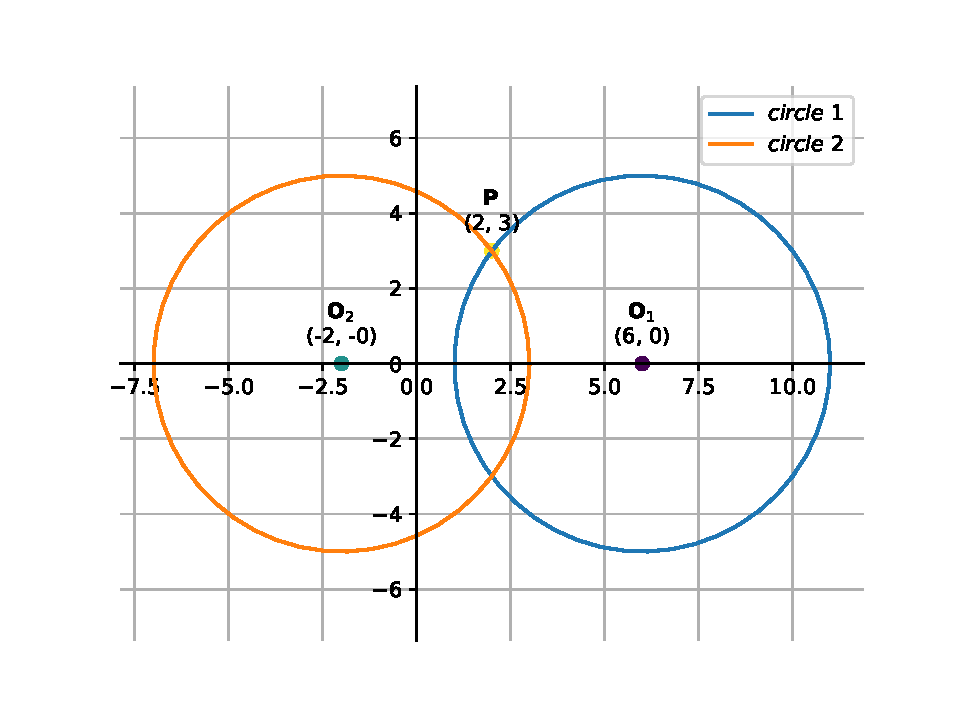
\includegraphics[width=0.75\columnwidth]{chapters/11/11/1/12/figs/fig.pdf}
		\caption{}
		\label{fig:11/11/1/12}
  	\end{figure}
From the given information, the following equations can be formulated
using 
	\eqref{eq:circ-eq}.
\begin{align}
		\label{eq:11/11/1/12/1}
	\norm{\vec{P}}^2 + 2 \vec{u}^{\top}\vec{P} + f &= 0
	\\
		\label{eq:11/11/1/12/2}
	\vec{u} &= k\vec{e}_1
	\\
		\label{eq:11/11/1/12/3}
	\norm{\vec{u}}^2 - f &= r^2
\end{align}
where 
\begin{align}
	\vec{P} = \myvec{2\\3} \text{ and } r = 5
\end{align}
From 
		\eqref{eq:11/11/1/12/1}
		and 
		\eqref{eq:11/11/1/12/3},
\begin{align}
	\norm{\vec{P}}^2 + 2 \vec{u}^{\top}\vec{P} + \norm{\vec{u}}^2 &= r^2
\end{align}
Substituting from 
		\eqref{eq:11/11/1/12/2} in the above, 
\begin{align}
	k^2  + 2k \vec{e}_1^{\top}\vec{P} + \norm{\vec{P}}^2- r^2 = 0
\end{align}
resulting in 
\begin{align}
	k =  - \vec{e}_1^{\top}\vec{P} \pm \sqrt{\brak{{ \vec{e}_1^{\top}\vec{P}  }}^2 + r^2 - \norm{\vec{P}}^2 } 
\end{align}
Substituting numerical values, 
\begin{align}
	k = 2, -6
\end{align}
resulting in circles with centre
\begin{align}
	-\vec{u} = \myvec{-2 \\ 0} \text{ or } \myvec{6 \\ 0}.
\end{align}
This is verified in Fig. 
		\eqref{fig:11/11/1/12}.
